\chapter{Phase d'analyse : des besoins aux fonctionnalités}
	\paragraph{}
	Dans la partie précédente nous avons vu ce qu'est un EAI et les enjeux de la
	supervision. Nous avons vu que TrackCIS est une console de supervision et
	notre projet vise à l'améliorer.
	Dans cette deuxième partie, nous chercherons à comprendre les besoins des
	utilisateurs de consoles de supervision et nous les traduirons en
	fonctionnalités implémentables dans TrackCIS.
	
	\subsection{L'enquête permet une meilleure compréhension des besoins des utilisateurs}
		\paragraph{}
		Un besoin est formulé par le destinataire d'une application, l'utilisateur. Il
		peut l'être explicitement ou implicitement. Dans le cas qui nous intéresse il
		nous importe de comprendre les besoins des utilisateurs potentiels de
		TrackCIS. De plus, pour véritablement comprendre ces besoins, nous devons
		aussi savoir qui sont les utilisateurs. L'enquête nous permettra d'obtenir ces
		informations.
		
		\subsubsection{Élaboration d'un questionnaire d'enquête et conduite des entretiens}
			\paragraph{}% Les objectifs de l'enquêtes
			L'enquête poursuit deux objectifs :
			\begin{itemize}
			  \item D’une part nous souhaitons pouvoir établir une liste de besoins.
			  \item D’autre part, cette enquête sera l’occasion de comprendre un peu
			  mieux comment sont organisés les DSIO (direction des services informatique
			  et de l’organisation) des établissements hospitaliers, ainsi que de faie
			  une typologie des utilisateurs de consoles de supervision.
			\end{itemize}
			
			\paragraph{}% Les grands thèmes abordés
			Pour répondre à ces deux objectif, le questionnaire d’enquête doit être le
			plus générale possible et les questions ouvertes. Ainsi, nous proposons le
			plan d'entretien suivant :
			\begin{itemize}
			  \item[1) Identification de la personne, exploration du contexte :] Cette
			  partie aura pour but de nous aider à comprendre comment est organisé le
			  service et qui est notre interlocuteur.
			  \item[2) Utilisations et utilisateurs de Cloverleaf et problématique de la
			  supervision des flux :] Dans cette partie nous poserons des questions sur
			  la manière dont est utilisé Cloverleaf et par qui ainsi que les personnes
			  qui sont en charge de la supervision.
			  \item[3) Attentes par rapport aux consoles de supervision :] Cette partie,
			  beaucoup plus abstraite, servira à comprendre ce qu’est la supervision
			  pour les utilisateurs de consoles et quels sont les attentes des
			  utilisateurs sur les consoles de supervision.
			  \item[4) Les consoles actuelles :] Ces questions viseront à explorer ce que
			  les utilisateurs utilisent le plus dans les outils existant, quels sont
			  les manques et les améliorations qu’ils proposent. Cette partie explorera
			  également les propositions des utilisateurs concernant un future module
			  statistique.
			\end{itemize}
			
			\paragraph{}% Conduite des entretiens
			Les entretiens sont conduit de manière semi-directive par téléphone ou en
			face à face quand cela est possible.
			Les questions présentent dans le guide d'entretien ne sont que des guides
			pour orienter la discussion, c’est pourquoi elles sont les plus ouvertes possible.\newline
			Le questionnaire a vocation à évoluer d’un entretien à un autre : des
			questions peuvent être modifiées, supprimées ou ajoutées de façon à obtenir
			des informations de plus en plus pertinentes (l'annexe 2 présente la dernière
			version du guide d'entretien). Chaque entretien donne lieu à un compte-rendu
			détaillé dont la structure reprend la trame du questionnaire.
			
			\paragraph{}% Les principes de l'étude qualitative
			Il s'agit d'une étude qualitative. Contrairement aux études quantitatives qui
			permettent de récolter des données repérsentatives d'une population donnée,
			dans une étude qualitative nous ne cherchons pas à interroger le plus de
			personnes possible. Les entretients sont basés sur des question ouverte et
			durent en général plus longtemp que dans des enquêtes quantitatives, une
			trentaine de minute dans notre cas.
			L'objetcif d'une telle étude est de faire ressortir la diversité des
			comportement. Ici, il s'agit entre autre de mettre en avant les différentes
			utilisations possibles des consoles de supervision et ses utilisateurs.
			
			\paragraph{}% Choix de la population interrogée
			Un panel de 5 établissements hospitaliers est interrogé. Tous ces
			établissements sont des clients d’Xperis :
			\begin{itemize}
			  \item Tour
			  \item Toulouse
			  \item Rouen
			  \item Brest
			  \item Metz
			\end{itemize}
			
			\paragraph{}% Méthodes d'analyse des résultat
			A l'issue des enquêtes nous procédons à l'analyse des résultats. Après une
			rapide relecture de tous les comptes rendu d'entretien, nous établissons une
			listes des grands thèmes qui ont été abordés durant les discussion.
			On classe ensuites chaque information collectée dans l'un de ces
			thèmes.\newline Les grand thèmes en question sont les suivants :
			\begin{itemize}
			  \item[- grand thème 1] L’organisation des services informatique dans les
			  hôpitaux,
			  \item[- grand thème 2] Les types d’utilisateurs de TrackCIS,
			  \item[- grand thème 3] Les types d’utilisations de TrackCIS,
			  \item[- grand thème 4] Les attentes par rapport aux consoles de supervision
			  et la réponse des outils actuels à ces attentes,
			  \item[- grand thème 5] Les fonctionnalités manquant aux consoles de
			  supervisions actuelles,
			  \item[- grand thème 6] Les statistiques sur les flux.
			\end{itemize}
			Dans la suite de cette partie nous entrerons dans le détail des informations
			collectées pour chacun de ces grand thèmes.
			
		\subsubsection{La supervision fait partie du processus de résolution des
		anomalies}
			\paragraph{}% Présentation
			Nous analysons ici l'organisation interne des services liées à
			l'interopérabilité dans les hôpitaux. Nous verons ensuite quelles sont les
			pratiques liées à la supervision (autrement dit, nous détaillerons les
			grands thèmes 1 et 3).
			
			\paragraph{}% L'organisation des DSIO
			Les services informatiques ont des structures très variables selon les
			établissements. Cependant, il existe dans tous les cas observés au moins un
			département consacré à l’interopérabilité. Ce département peut se subdiviser
			en deux pôles :
			\begin{itemize}
			  \item Un pôle intégration,
			  \item Un pôle exploitation
			\end{itemize}
			\textbf{Le pôle intégration} prend en charge la mise en place de nouveaux
			flux et du bon fonctionnement de l’EAI en général. Son niveau de compétence sur
			Cloverleaf est élevé. Ce type de pôle existe dans des établissements
			relativement autonomes vis-à-vis des éditeurs de logiciels. Le pôle
			intégration se compose généralement de 2 à 3 personnes. Les outils utilisés
			sont principalement l’IDE, et des consoles de supervision telles que EAI
			Supervision ou Global Monitor.\newline
			\textbf{Le pôle exploitation} a en charge la supervision des flux. Le niveau
			de maîtrise de Cloverleaf y est plus faible. Les outils utilisés sont en
			général les différentes consoles de supervision,
			mais rarement l’IDE, trop complexe pour ce type d’utilisateur.\newline
			Les deux pôles peuvent cohabiter au sein d’un même établissement. Certains,
			comme le CHU de Metz, n’ont qu’un pôle exploitation, la mise en place des
			flux étant assuré par un autre département (en l’occurrence, le département
			en charge de l’urbanisation du SI). D’autres établissements, beaucoup plus
			dépendants des éditeurs, ne s’occupent pas de la mise en place des flux ni
			du fonctionnement de l’EAI, mais seulement de la supervision. C’est par
			exemple le cas du CHU de Châtellerault.\newline
			La figure \ref{orga_interop} résume les différents niveaux de gestion de
			l’interopérabilité au sein d’un hôpital. Les niveaux correspondent au degré
			de responsabilité vis à vis de l'interopérabilité. Plus un niveau est élevé,
			plus les impactes des décisions prises à ce niveaux seront fort sur le SI. Un
			pôle exploitation se situe au niveau le plus bas tandis qu’un pôle
			intégration peut se situer au niveau 2 ou 3. Le niveau le plus haut est en
			général assuré par un département urbanisation, en charge de la définition
			de la politique de tout le SI.
			% Niveau de responsabilité pour l'interop dans le SI
			\begin{figure}[H]
				\centering
				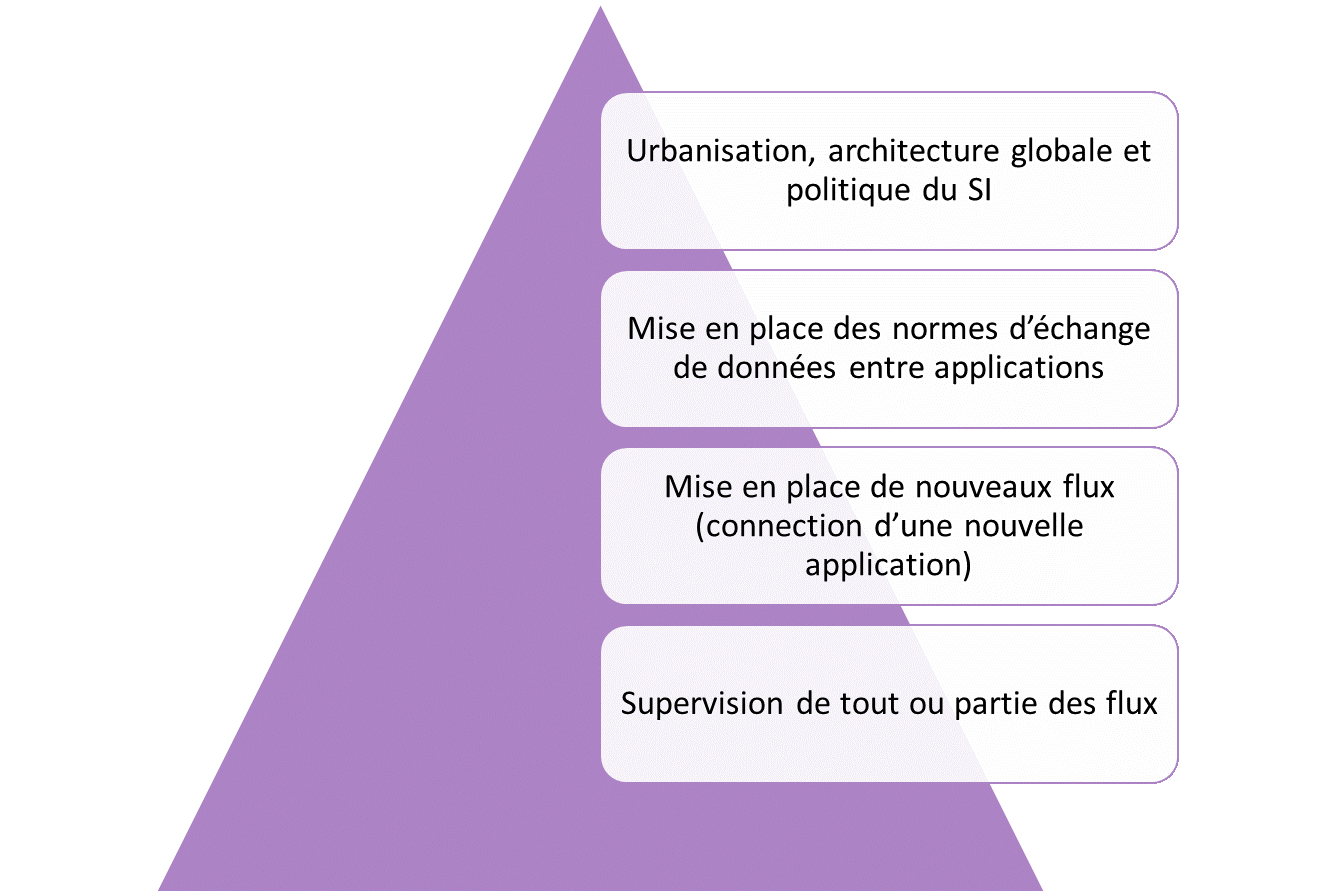
\includegraphics[width=8cm]{../img/si_1.png}
				\caption{\label{orga_interop} Les différents niveaux de responsabilité
				autour de la gestion de l'interopérabilité.}
			\end{figure}
			
			\paragraph{}% Diversité des pratiques
			L’ensemble des outils liés à Cloverleaf (IDE et consoles de supervision)
			sont utilisés pour la supervision des flux. Les utilisateurs les plus
			aguerris sur Cloverleaf utilisent l’IDE, notamment à une fonctionnalité,
			nomée \textit{status}, qui donnes accès à des données statistiques sur un
			thread ou un process à un instant t. Pour détecter les problèmes,
			l’utilisateur se fie principalement à la date et heure de dernière écriture
			d’un message sur le flux. Si rien n’a été écrit depuis un certain temps, c’est que
			le flux est bloqué et que les messages ne passent plus. Ce type d’utilisateur est
			généralement en charge de la résolution des problèmes les plus complexes.
			Pour cela, il a parfois recours à des fonctionnalité avencées comme la
			consultation de la base de donnée d'erreur (ou \textit{error database}) ou
			à base de données contenant les messages pour comprendre l’origine de
			l’erreur.\\
			Du côté des consoles de supervision, les usages qui sont ressortis sont :
			\begin{itemize}
			  \item Visualiser l’état des flux (si les threads et process sont bien en
			  marche),
			  \item Affichage sur écran géant,
			  \item Rechercher un message en particulier, ou un certain type de
			  messages. Par exemple, tous les messages concernant un patient donné,
			  \item Visualiser les messages en erreur,
			  \item Supervision en mode lecture seule : vérifier que les messages
			  passent bien et connaître l’origine des erreurs,
			  \item Explorer le contenu des messages pour diagnostiquer une erreur,
			  \item Réaliser des tests lors de la mise en place de flux (usage repéré
			  uniquement au CHU de Toulouse),
			  \item Editer le contenu des messages en cas d’erreur,
			  \item Rejouer des messages après les avoir édités,
			  \item Pour les flux Maincare et EAI Supervision, s’assurer que les
			  messages sont bien intégrés dans les applications de destination,
			  \item Restreindre l’utilisation de certaines fonctionnalités pour par
			  exemple confier les outils à des personnes d’astreintes ou des personnes
			  métier,
			  \item Comparer le contenu d’un message entre son entrée dans un flux et
			  sa sortie. Cet usage n’a été référencé que pour EAI Supervision,
			  \item Paramétrer l’outil : création de colonnes, attribution des droits…
			\end{itemize}
			\paragraph{}
			Cette liste nous permet de connaître les principales utilisations des
			consoles de supervision (figure \ref{usage_consoles}). L’utilisation la plus
			simple est la visualisation : voir les messages qui passent et pouvoir détecter rapidement
			les erreurs. Une fois les erreurs détectées, l’utilisateur cherche à
			comprendre ce qui les a causées. Pour cela, il peut être suffisant de
			regarder le contenu du message pour en repérer les anomalies, ou bien aller
			dans l’error database. Une fois la cause de l’erreur bien établie, vient une
			phase de correction. Celle-ci peut se faire par édition du contenu du
			message et par rejoue, dans les cas les plus simples. Comme c’est le cas
			pour le CHU de Toulouse, la console peut être utilisée pour effectuer des
			tests lors de la mise en place de nouveaux flux. C’est-à-dire vérifier que
			les messages passent correctement d’une application à une autre. Enfin, les
			utilisateurs les plus avertis ont en charge l’administration de la console,
			c’est-à-dire son paramétrage (attribution des droits de consultation et
			d’action aux utilisateurs, paramétrage des données affichées\ldots). Ce rôle
			revient généralement au pôle intégration, aux éditeurs ou à Xperis. On
			remarque que, dans le cas de TrackCIS, le paramétrage de la console est un
			facteur limitant à son utilisation en production.
			\begin{figure}[H]% Niveau de responsabilité pour l'interop dans le SI
				\centering
				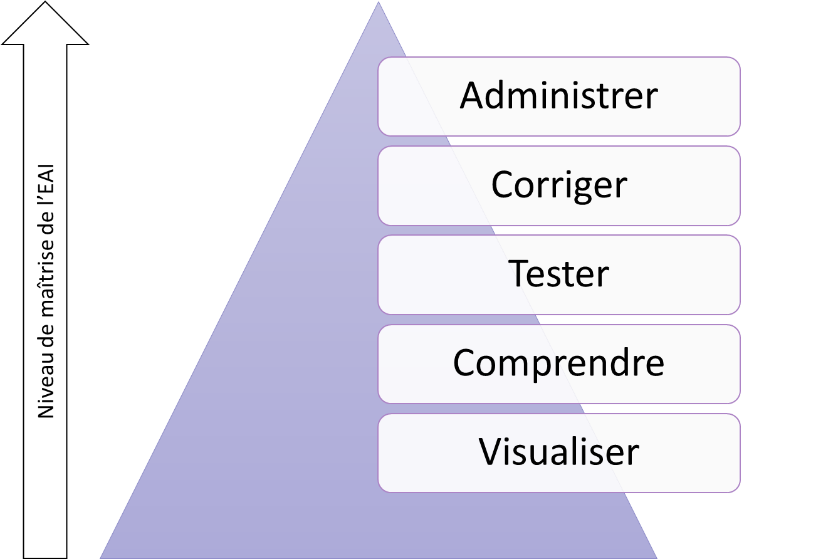
\includegraphics[width=10cm]{../img/usage_1.png}
				\caption{\label{usage_consoles} Les différentes utilisations des consoles
				de supervision.}
			\end{figure}
			
			\paragraph{}
			En résumé, nous pouvons définir la supervision d'un flux comme :
			\begin{itemize}
			  \item Détecter en un coup d’œil la présence d’anomalies telles que :
			  	\begin{itemize}
			  	  \item Des erreurs,
			  	  \item Des ralentissements,
			  	  \item Des blocages
		  	    \end{itemize}
			  \item Pouvoir expliquer, même partiellement ces anomalies,
			  \item Et éventuellement pouvoir agir dessus dans le but de les corriger,
			  par exemple en rejouant un message qui n’est pas passé à cause d’un
			  problème momentané de la connexion. Selon deux des 5 personnes interrogées,
			  le but premier d'une console de supervision n'est cependant pas la
			  correction de anomalie, mais uniquement leur détection.
			\end{itemize}
			
		\subsubsection{Une grande diversité des utilisateurs des consoles de
		supervision}
			\paragraph{}% Présentation
			Nous savons maintenant comment à lieux la superision d'un flux dans la
			pratique et nous connaissons un peu mieux l'organisation en place dans les
			centres hospitaliers. Nous présenterons ici la typologie des utilisateur qui
			est ressortie de l'étude, ce qui correspond au grand thème 2.
			
			\paragraph{}% Les utilisateurs
			La typologie des utilisateurs découle du schéma d’organisation des services
			informatiques vu préciédemment (figure \ref{orga_interop}. On retrouve les
			deux niveaux que sont l’intégration et l’exploitation en plus d’un troisième
			niveau : le niveau métier. Le tableau \ref{type_utilisateurs} propose une
			description des 4 grands profils d’utilisateurs de consoles de supervision que l’étude a dégagée.
			\begin{table}[H]
				\centering
				\begin{tabular}{| p{3cm} | p{4,5cm} | p{4,5cm} | p{4,5cm} |} %Exemples des
				% principaux logiciels métier
					\hline
						\thead{Utilisateur}
						&\thead{Niveau de maitrise}
						&\thead{Outils utilisés}
						&\thead{Rôles}
						\\
					\hline
						Responsable d'intégration
						&
						Bon niveau de maîtrise de Cloverleaf.
						&
						Tous les outils (l'IDE, EAI Supervision, Global Monitor et TrackCIS)
						&
						Mise en place de nouveaux flux, résolution des problèmes complexes.
						\\
					\hline
						Responsable d'exploitation
						&
						Connaissances et formation de base sur l’EAI.
						&
						Consoles de superivision (EAI Supervision, Global Monitor et TrackCIS)
						&
						Surveillance, correction des erreurs simples (erreurs de contenus de
						messages), remonte les erreurs plus complexes
						\\
					\hline
						Personne d'astreinte
						&
						Il s'agit en général d'informaticiens mais non spécialisés et non formés
						sur Cloverleaf.
						&
						Consoles de supervision simples d'utilisations telles que TrackCIS ou
						Global Monitor.
						&
						Surveillance de quelques flux et éventuellement correction des erreurs les
						plus simples.
						\\
					\hline
						Référent applicatif
						&
						Pas ou peu de connaissance sur le fonctionnement de Cloverleaf. Il s'agit
						malgré tout de profils informaticiens.
						&
						Des consoles de supervision simple d'utilisation telle que TrackCIS.
						&
						Surveiller les flux concernant une application dont ils ont la charge. Les
						référents applicatifs existent déjà dans les hôptitaux, mais ils ne
						s'occupe pas de l'interopérabilité.
						\\
					\hline
						Référent métier
						&
						Pas de connaissances sur le fonctionnement de l’EAI. Typiquement il s'agit
						de personnel médical (infirmière, pharmacien\ldots) ou administratif.
						&
						Des consoles de supervision simple d'utilisation telle que TrackCIS.
						&
						Surveillance et éventuellement correction des erreurs simples. Ce type
						d'utilisateur n'existe pas encore dans les hôpitaux. Cependant, 3 des 5
						établissements interrogés disent avoir la volonté de mettre en place ce
						type d'utilisateur.
						\\
					\hline
				\end{tabular}
				\caption{\label{type_utilisateurs} Typologie des utilisateur dégagée par
				l'enquêtes.}
			\end{table}
			Ces différents acteurs coopèrent ensemble pour la résolution de problème,
			comme le résume la figure \ref{resolution_pbs}. Ce processus fait intervenir
			beaucoup d’intermédiaires ce qui pose problème à la fois aux utilisateurs métiers,
			car la résolution de problème prend du temps, et au services informatiques
			(notamment les pôles intégration et exploitation) car ils se retrouvent à
			devoir régler quotidiennement des problèmes parfois simple (comme des
			erreurs de saisie). Ceci justifie la volonté de certains établissements,
			comme le CHU de Toulouse, de donner accès à des utilisateurs métiers
			d’applications la possibilité de corriger les erreurs les plus simples
			(comme les erreurs de saisie).
			\begin{figure}[H]
				\centering
				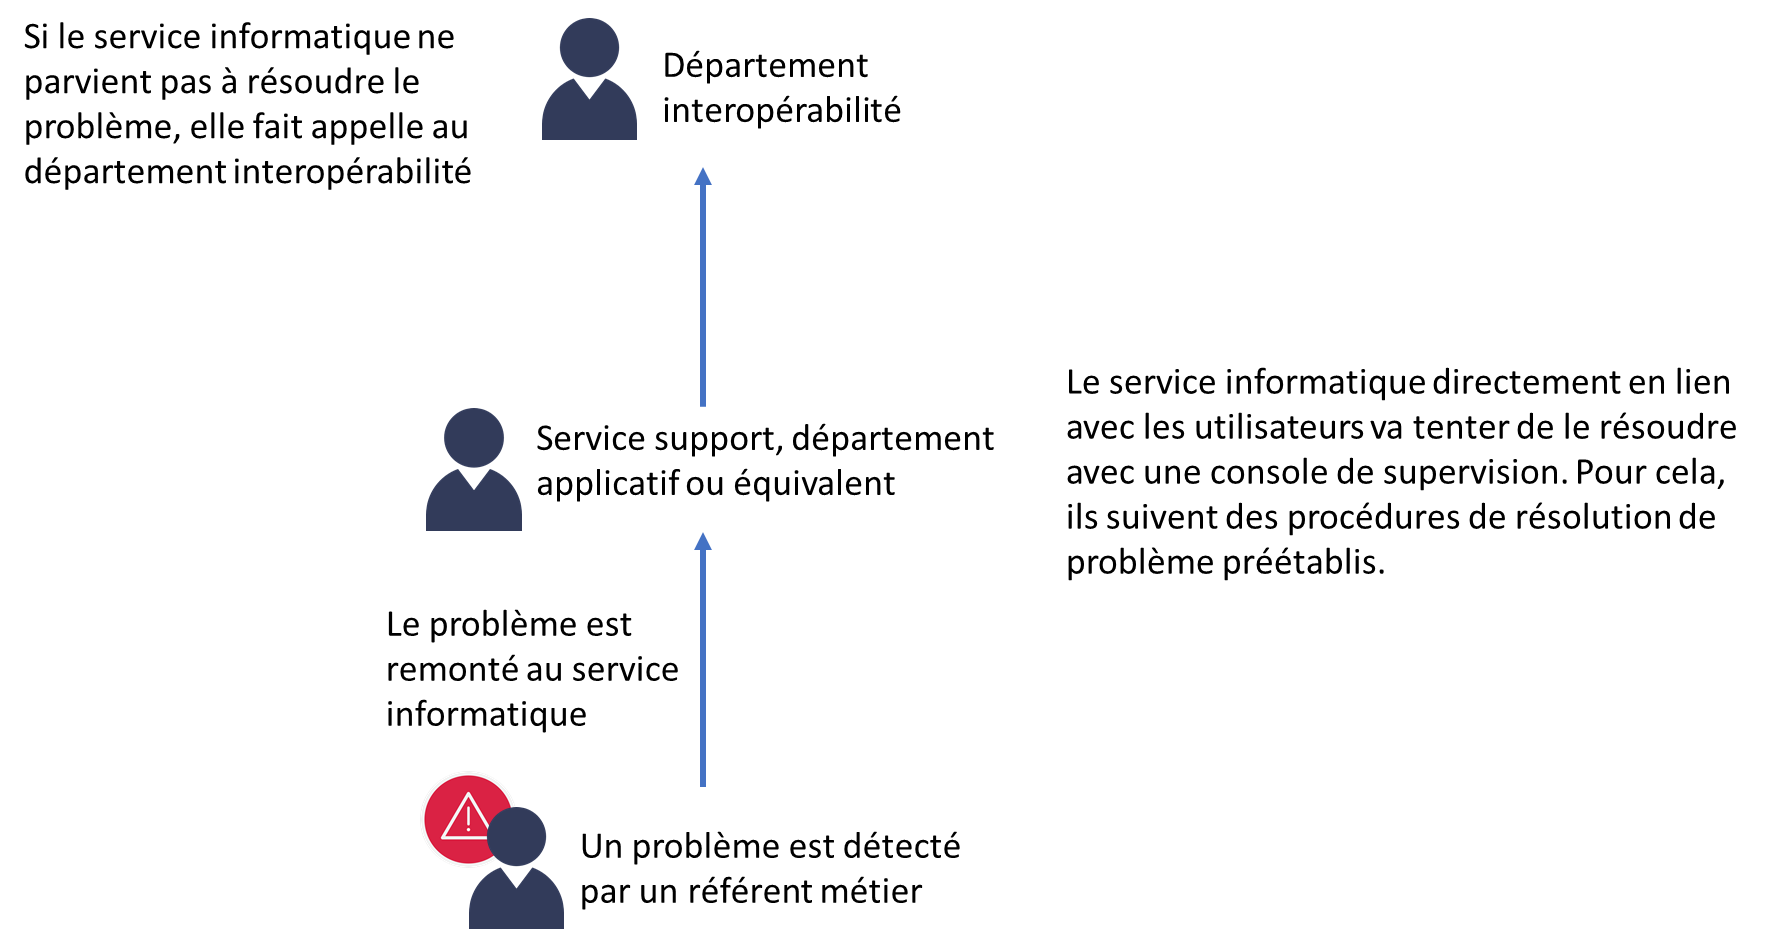
\includegraphics[width=15cm]{../img/user_1.png}
				\caption{\label{resolution_pbs} Processus de résolution d'un problème dans
				Cloverleaf.}
			\end{figure}
			
		\subsubsection{L'enquête permet de dresser une liste des besoins}
			\paragraph{}% Les attentes qui sont ressorties de l'enquête
			Nous remarquons que les avis concernant le rôle des consoles de supervisions
			convergent entre les différentes personnes interrogées. Celles-ci attendent
			de ces outils qu’ils jouent le rôle de tableau de bord clair, simple et si
			possible au design épuré de façon à ce que les informations soient les plus
			lisibles possibles. Une console doit permettre une visualisation rapide des
			erreurs. Elles doivent également permettre leur analyse. La correction des
			erreurs n’est évoquée que comme une fonction secondaire et facultative de
			ces outils.\newline
			D’une manière générale, les utilisateurs son satisfait de l’ergonomie de TC.
			Les principales remarques concernant ce point sont :
			\begin{itemize}
			  \item Le paramétrage des colonnes qui est difficile,
			  \item La lenteur d’affichage des messages,
			  \item Pour certains flux  (les flux externes), il faut parcourir tous les
			  messages pour retrouver ceux ayant un retour négatif.
			\end{itemize}
			Le ressenti global est que les utilisateurs informaticiens, principalement du
			département interopérabilité, ne sont pas spécialement sensibles à
			l’ergonomie des outils de supervision. Ils sont plus soucieux du fonctionnel
			que du design. Mais la plupart des personnes interrogées soutiennent que des
			utilisateurs métiers seraient, quant à eux, plus soucieux du design et de la
			facilité de prise en amin de l’outil. Malheureusement, nous n’avons pu
			interroger de tels utilisateurs.
			
			\paragraph{}% C'est quoi une bonne console
			En résumé, une bonne console est un outil donnant la vision la plus générale
			possible. La console de supervision a pour objectif premier de faire gagner
			du temps à son utilisateur et à permettre une résolution plus rapide des
			problèmes. De ce fait, la console de supervision a pour objectif d’améliorer
			la fiabilité globale de l’EAI, donc du SI.
			
			\paragraph{}% La lise des besoins, classification
			En plus des information que nous avons décrites jusque là, les entetiens nous
			on permi de faire remonter différents besoins des utilisateurs. Ceux-ci l'ont
			été explicitement ou non, et concerne généralement des manques. Voici
			quelques exemples de besoins, la liste complète se trouvant en annexe 3 :
			\begin{itemize}
			  \item Pouvoir trouver facilement la cause des erreurs,
			  \item Voir l'évolution du nombre de messages envoyés par flux au cours du
			  temps,
			  \item Voir la date et heure d'écriture du dernier message,
			  \item Visualiser l'état des flux en temps réel,
			  \item Pouvoir afficher la console sur un écran géan
			\end{itemize}
			Un total de 57 besoins ont été ainsi identifié. Ceux-ci ne sont pas
			spécifiquements lmié à un outil en particulier, ils concernent la supervision
			en général. Certains de ces besoins son d'ailleurs déjà satisfait dans
			TrackCIS, comme c'est par exemple le cas pour : "Pouvoir rejouer les
			messages" ou encore "Avoir un outil utilisable en lecture seule". Ce type de
			besoin nous ayant été remonté par des non utilisateurs de TrackCIS. Nous
			pouvons faire un premier classement des besoins en utilisant les catégories
			suivantes :
			\begin{itemize}
			  \item Besoins concernant les performances,
			  \item Besoins concernant le design, l'ergonomie et la facilité
			  d'utilisation,
			  \item Besoins concernant la résulution des problèmes,
			  \item Besoins concernant les données statistiques,
			  \item Besoins concernant les rôles de la console,
			  \item Les autres besoins
			\end{itemize}
			
			\paragraph{}% Mode de passage des besoins aux fonctionnalités
			Grace à l'enquête terrain, nous en savons un peu plus sur le mode de
			fonctionnement de l'interopérabilité dans le monde hospitalier. Nous en
			savons également d'aventage sur la supervision et les pratiques associée
			ainsi que les paersonnes qui en ont la charge. Enfin, nous avons une liste de
			besoins liés à la supervision des flux. Il est important de préciser que
			nous ne traiterons pas ici tous les besoins de cette liste, mais uniquement
			ceux relatifs à un module statistiques.
			Ce choix est justifié par le fait que :
			\begin{itemize}
			  \item Certain des besoins listés sont déjà satisfait par TrackCIS. En
			  effet, les questions posées lors des entretiens n'étaient pas
			  spécifiquement portées sur cet outil, la plupart des personnes interogées
			  ne l'utilisant pas. Ces besoins ne seront donc pas traités.
			  \item Xperis souhaite apporter toutes les améliorations nécessaires à
			  TrackCIS. Cependant, l'amélioration prioritaire concerne le nouveau module
			  statistique. C'est pourquoi les besoins ayant atrait aux statistiques
			  seront les seuls à être tratiés ici, et donc à être déclinés en
			  fonctionnalités.
			\end{itemize}
			Les élements de cette liste qui ne seront pas traités dans ce mémoire
			pourront servir de base à Xperis pour des amélioration future de l'outil.
			
			\paragraph{}% La lise des besoins, priorisation
			Le classement des besoins permet d'en faciliter la lecture et la
			compréhension, ce qui nous permettra d'imaginer plus aiséement les
			fonctionnalités qui viendrons y répondre. De plus, tous les éléments de cette
			liste ne sont pas égaux, certains besoins compte d'avantage aux yeux des
			personnes interrogée que d'autre. De plus certains ont été cité plus souvant.
			L'enquête que nous avons mené est qualitative et le faible panel de personnes
			interrogées ne nous permet pas de faire des analyse statistiques sur la
			récurence de certains besoins. Cependant, ledit panel est représentatif des
			utilisateurs actuels de TrackCIS, qui ont tous été interrogés. De façon à
			noter l'inportance de chaque besoin pour les utilisateurs, nous proposons de
			nous baser sur le barème présenté dans le tableau \ref{bareme_besoins}
			ainssi que sur le nombre de citation. Le choix des notes dans le barème
			ci-dessous est arbitraire et a pour but de bien différencier les besoins les
			plus prioritaires de ceux qui le sont moins.
			\begin{table}[H]
				\centering
				\begin{tabular}{| p{4cm} | p{8cm} | p{2cm} |}
					\hline
						\thead{Priorité}
						&\thead{Description}
						&\thead{Note}
						\\
					\hline
						Peu important
						&
						S'il est satisfait, ce besoin ne fait qu'améliorer le confort de l'utilisateur. S'il ne l'est pas, rien ne change.
						&
						2
						\\
					\hline
						Important
						&
						S'il est satisfait, améliore l'efficacité de l'utilisateur dans son métier
						&
						3
						\\
					\hline
						Très important
						&
						S'il est satisfait, améliore considérablement l'efficacité de l'utilisateur dans son métier
						&
						5
						\\
					\hline
						Critique
						&
						Besoin qu'il est nécessaire de satisfaire, faute de quoi cela nuira à l'utilisateur.
						&
						8
						\\
					\hline
				\end{tabular}
				\caption{\label{bareme_besoins} Barème choisi pour noter l'importance de
				chaque besoin perçue lors de l'entretien.}
			\end{table}
			Nous calculons la note de chaque besoin avec la formule ci-dessous
			(\ref{besoin_formule}).
			Soit N le nombre de citation et I la note d'importance définie avec le barème du
			tableau \ref{bareme_besoins}.
			\begin{equation}
				\label{besoin_formule}
				Note\ du\ besoin=N\times I
			\end{equation}
			Le résultat de cette priorisation se trouve dans la colonne "Note besoin" du
			tableau de l'annexe 3.
	
	\subsection{La liste des besoins permet de dresser une liste de fonctionnalités}
		\paragraph{}% On ne se concentre que sur les besoins liés aux stats
		Nous avons dressé et analysé une liste de besoins émanant d'utilisateur
		concernant la supervision. L'objectif est maintenant, à partir de cette liste,
		de dresser une liste de fonctionnalités.
		
		\subsubsection{De la liste des besoins à la liste des fonctionnalités}
			\paragraph{}% C'est quoi une fonctionnalité ??
			Une fonctionnalité est un service rendu par une application à un utilisateur.
			Par exemple, la version actuelle de TrackCIS permet à l'utilisateurs de
			consulter la liste des messages qui sont passé dans un flux. Ceci est une
			fonctionnalité et elle répond à un besoin de l'utilisateur. En l'occurence le
			besoin en question pourrait être "consulter la liste des messages transitant
			par le fux". Dans ce cas-ci, le passage du besoin à la fonctionnalité est
			évidente, puisque ls deux sont formulable de la même manière. Mais dans ce
			cas quelle est la différences entre les deux ? Un besoin n'est pas lié à un
			outil en particulier, c'est une volonté de l'utilisateur lié à un manque. Une
			fonctionnalité est elle liée à un outil particulier, puisqu'il s'agit d'un
			service rendu par cet outil.
		
			\paragraph{}% La liste des fonctionalités
			On peut établir des fonctionnalités à partir des besoins que l'on a retenu.
			Une fonctionnalité est une réponse à un besoin. Cette réponse est portée par
			un outil, en l'occurence TrackCIS. Les besoins retenus sont aux nombre de 33.
			Nous imaginons à partir de là une liste composée de 30 fonctionnalités
			(annexe 4) regroupées en 8 grands ensembles :
			\begin{itemize}
			  \item Visualisation du niveau de disponibilité du flux.
			  \item Visualisation de la date et heure du dernier message passé.
			  \item Visualisation de l’historique des messages.
			  \item Visualisation des ressources serveur.
			  \item Administration des statistiques.
			  \item Exporter les données statistiques.
			  \item Facilitation de l’utilisation.
			\end{itemize}
			
		\subsubsection{Priorisation des fonctionnalités liées aux statistiques}
			\paragraph{}% But de la priorisation des fonctionnalités
			De la même manière que nous avons priorisé les besoin, nous cherchons ici à
			prioriser les fonctionnalités qui en découlent. L'objectif de cela est
			d'anticiper le développement des fonctionnalités : les plus importantes
			devant être implémentées en premier. Il nous faut donc mettre en place un
			barème permettant d'ordonner les fonctionnalités les unes par rapport aux
			autres. Nous allons nous ader pour cela du diagramme FODA (Feature Oriented
			Domain Analysis).
			
			\paragraph{}% Présentation FODA
			Le diagramme FODA est une représentation graphique des différentes
			fonctionnalités de l’application (Kang, 1990). Il est organisé en features.
			Une feature est une macro fonctionnalité. A l’intérieur de chaque feature
			peuvent se trouver d’autres fonctionnalités, plus précises, sous lesquelles
			peuvent s’en trouver d’autres, etc. Les feuilles de l’arbre ainsi formé
			(correspondant au niveau de fonctionnalité le plus détaillé) correspondent à
			des parties fonctionnelles de l’application qui seront développées.\newline
			La figure \ref{foda_legende} présente le principe de base du diagramme FODA.
			La \textit{feature} 1 est obligatoire (point noir), elle correspond à la
			fonctionnalité d'un produit minimum viable (PMV). La \textit{feature 2} est
			facultative (point blanc), elle correspond à une fonctionnalité qui pourra être
			développée dans des versions plus évoluées ou plus personnalisées de
			l’outil. Elle n’est pas indispensable au fonctionnement ni à la mise sur le
			marché, mais rend tout de même un service intéressant pour l'utilisateur.
			\begin{figure}[H]% Légende du FODA
				\centering
				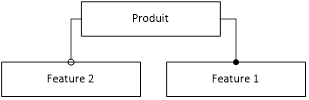
\includegraphics[width=7cm]{../img/foda_legende.png}
				\caption{\label{foda_legende} Principe du diagramme FODA.}
			\end{figure}
			
			\paragraph{}% FODA de TrackCIS stats
			Nous mettons en pratique cette classification en concertation avec l'équipe
			d'Xperis. Cette séparation entre fonctionnalité optionnelles ou faisant parti
			du PMV refète donc le choix de l'entreprise. Pour tenir également compte des
			priorités des utilisateurs interrogés durant l'enquête, nous proposons la
			formule ci-dessous. Soit Bi la note d'un besoin donnée,
			\begin{math}\sum Bi\end{math} représente la somme des notes des besoins qui
			sont satisfaits par cette fonctionnalité. On a la formule \ref{fonctio_nopmv}
			pour une fonctionnalité notée comme facultative et la formule
			\ref{fonctio_pmv} pour une fonctionnalité notée comme obligatoire. Les notes
			obtenues pour chaque fonctionnalités sont présentées dans la colonne "Note
			de fonctionnalité" du tableau de l'annexe 4.
			\begin{equation}
				\label{fonctio_nopmv}
				Note\ de\ la\ fonctionnalite=\sum Bi
			\end{equation}
			\begin{equation}
				\label{fonctio_pmv}
				Note\ de\ la\ fonctionnalite=2\times \sum Bi
			\end{equation}
			
		\subsubsection{Le nouveau module se découpe en huits grands groupes de
		fonctionnalités}
			\paragraph{}
			Les figures \ref{foda_1} et \ref{foda_2} représentent l'ensemble des
			fonctionnalités du module statistique de TrackCIS sous forme de diagramme
			FODA . Chaque feature correspond à un des 8 grands
			ensembles de fonctionnalité décrit précédemment.\newline
			La page dédiée aux statistique serait divisée en widgets. Chacun est une
			petite boite contenuant un type d'informations. Dans la version que nous
			proposons ici, ils sont au nombre de cinq et correspondent aux features
			décrites ci-dessous.
			\begin{figure}% foda 1
				\centering
				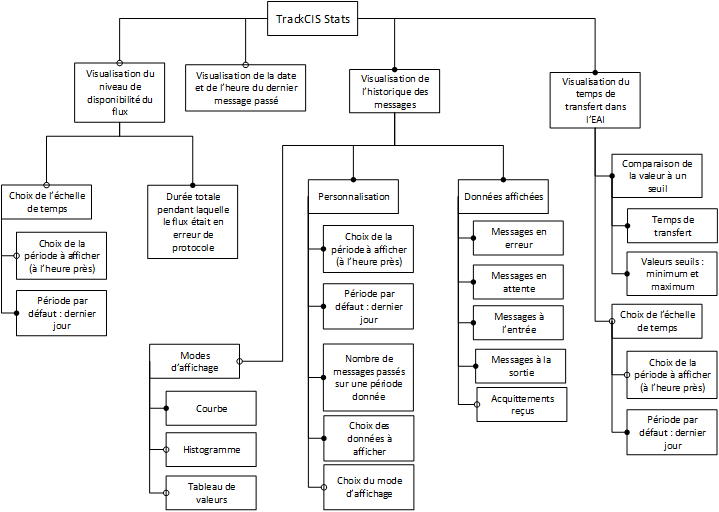
\includegraphics[width=17cm]{../img/part2/foda_1.png}
				\caption{\label{foda_1} Diagramme FODA pour le module statistique de
				TrackCIS (première partie).}
			\end{figure}
			\begin{figure}% foda 2
				\centering
				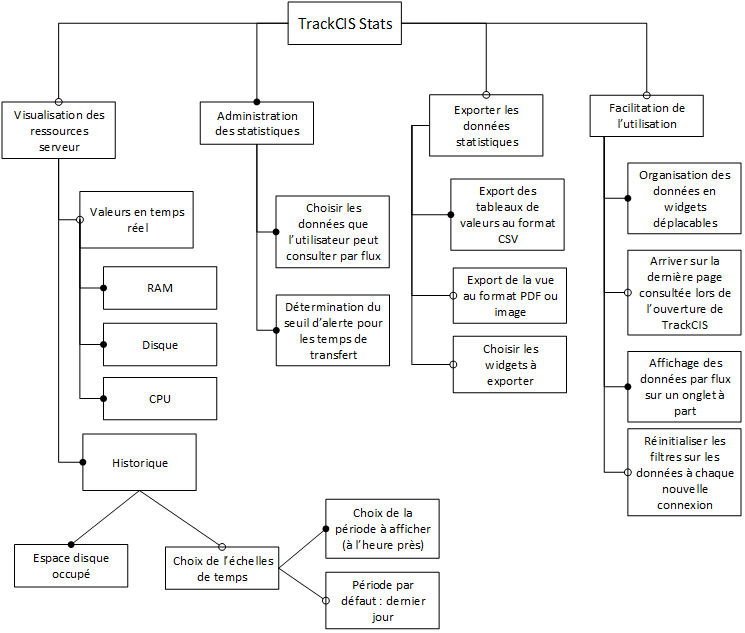
\includegraphics[width=17cm]{../img/part2/foda_2.png}
				\caption{\label{foda_2} Diagramme FODA pour le module statistique de
				TrackCIS (deuxième partie).}
			\end{figure}
			
			\paragraph{Visualisation du niveau de disponibilité du flux.}
			Cette feature correspond au widget permettant d'afficher le taux de
			disponibilité du flux. Il s'agit du ratio entre le temps de bon
			fonctionnement du flux sur le temps où celui-ci ne fonctionnait pas pour
			causes d'erreurs. Cet indicateur permet de détecter rapidement les flux les
			plus problématiques. Cette valeur serait calculée sur une période de temps
			définie par l'utilisateur.
			
			\paragraph{Visualisation de la date et heure du dernier message passé.}
			Il s'agit d'une fonctionnalité toute simple mais que l'étude du besoin a fait
			ressortir comme importante. Il s'agit d'un petit widget indiquant avec
			précision la date et l'here à laquelle un message est correctement passé pour
			la dernière fois sur ce flux. Ceci est un bon indicateur du bon
			fonctionnement d'un flux. Dans la plupart des flux hospitaliers, des messages
			passent en permanance. Le fait qu'il n'en passe pas pendant un certain temps
			est révélateur de problèmes.
			
			\paragraph{Visualisation de l’historique des messages.}
			Cette feature correspond à un widget affichant l'historique du nombre de
			messages passés sur le flux. Celui-ci peut prendre la forme d'une courbe,
			d'un histograme ou d'un simple tableau de valeurs. L'utilisateur choisi la
			période qu'il veut visualiser ainsi que les types de données. Ce widget
			permettrait de voir l'évolution au cours du temps des messages ayant
			correctement transité dans le flux, des messages tombés en erreurs ou en
			attente ou encore des acquitements ressuent des applications destinataires.
			
			\paragraph{Visualisation des ressources serveur.}
			Cette feature correspond à deu widgets qui ont tous deux atrait à l'état du
			serveur sur lequel est installé Cloverleaf. Le premier d'entre eux permet
			d'avoir des information sur l'état en tant réel du serveur : occupation de la
			mémoire vive et du disque, utilisation du processeur. Le deuxième widget
			permet de voir l'évolution au cours du temps de l'occupation du disque du
			serveur. Cette donnée présentée sous la forme d'une courbe, peut permetre
			d'identifier une augmentation anormal de l'espace occupé, ce qui peut
			correspondre à une mauvaise gestion de la mémoire au niveau de l'EAI, ce qui
			peut poser problème à terme.\newline
			Les deux dernières features ne correspondent à aucun widget sur l'onglet
			statistiques.
			
			\paragraph{Administration des statistiques.}
			Cette partie est réservée aux administrateurs. Il s'agit d'un nouvel Dans le
			PMV il est possible de définir quel utilisateur peut voir quel widget sur sa
			page statistique. Ce qui signifie que l'utilisateur ne peut pas paramétrer
			sa propre page, a part la position des widgets.
			
			\paragraph{Exporter les données statistiques.}
			L'utilisateur doit pouvoir exporter les données qu'il voit sur sa page
			statistique. L'export se fait donc pour un flux donné et dans divers formats.
			Dans le PMV, il est uniquement possible d'exporter les données sous forme de
			PDF ou d'image reprenant l'affichage du contenu des widgets à l'identique.
			Une version plus évoluée de la feature permettrai de choisir quelles sont les
			widget que l'on veut exporter, s'il faut qu'ils le soit chacun sur un fichier
			séparer.
			
			\paragraph{Facilitation de l’utilisation.}
			
	
	\subsection{Des fonctionnalités vers les cas d'utilisation}
		\paragraph{}
		Nous savons maintenant quelles sont les services que doit rendre notre nouveau
		module.
		
		\subsubsection{État de l'art sur les consoles de supervision et la visualisation de données}
			\paragraph{}
			Pour cet état de l’art nous nous baserons sur des outils remplissant des
			fonctions similaires à celles que l’on attendrait de TrackCIS. Cet état de
			l’art est réalisé dans le but du développement du module statistique. Nous
			nous attarderons donc, dans l’analyse des exemples, sur :
			\begin{itemize}
			  \item Les données qui sont affichée et leurs rôles,
			  \item La manière dont ces données sont représentées (courbe, histogramme,
			  jauge...), pourquoi elles sont représentées de la sorte et si cela semble
			  efficace et ergonomique du point de vue de l’utilisateur.
			\end{itemize}
			Nous analyserons ici 2 outils : TradeXpress et M12.
			
			\paragraph{TradeXpress :}
			TradeXpress est une plateforme d’intégration B2B. L’outil permet de connecter
			les application d’une entreprise à celles de ses partenaires (clients,
			fournisseurs…). TradeXpress n’est pas spécialisé dans un domaine en
			particulier. Il permet de gérer l’intégralité des flux, il va bien au-delà
			de la simple supervision. Cependant, certaines de ces fonctionnalités sont
			axés supervision, ce sont celles qui nous intéressent ici. La figure
			\ref{trade_xpress} présente la page de monitoring des flux de la console.\newline
			La vue se divise en deux parties aux rôles différents : une partie consacrée
			à l’état du système, une autre dédiée à la supervision. La première partie
			montre une vision de l’état actuel (en temps réel) du serveur. La partie
			supervision offre deux vision :
			\begin{itemize}
			  \item Une au jour à l’aide de jauges montrant le nombre de messages ou
			  documents transitant par l’EAI. On peut voir juste en dessous de l’encadré
			  gris un bouton permettant de sélectionner la date.
			  \item Un historique à la semaine du volume de messages passés pour chaque
			  domaine. L’utilisateur peut choisir les données ainsi que la semaine à
			  afficher.
			\end{itemize}
			Le design de l’outil est simple et relativement classique. Les informations
			utiles à l’utilisateur occupent un maximum de place sur la page. Il y a le
			moins de superflu possible : pas de cadre autour des parties et seulement
			cinq couleurs différentes.\newline
			Pour la partie supervision, l’utilisateur ne peut pas sélectionner la
			période de temps, il doit se contenter de visualiser les données d’un jour
			ou d’une semaine particulière. Ceci restreint les possibilités de
			visualisation, mais simplifie l’utilisation de la console.\newline
			Pour que les jauges soient pertinentes il faut qu’elles soient calibrées avec
			une valeur minimum et maximum. La documentation disponible en ligne ne précise
			pas s’il est possible de calibrer ces jauges, ni à qui revient ce rôle.
			\begin{figure}[h]
				\centering
				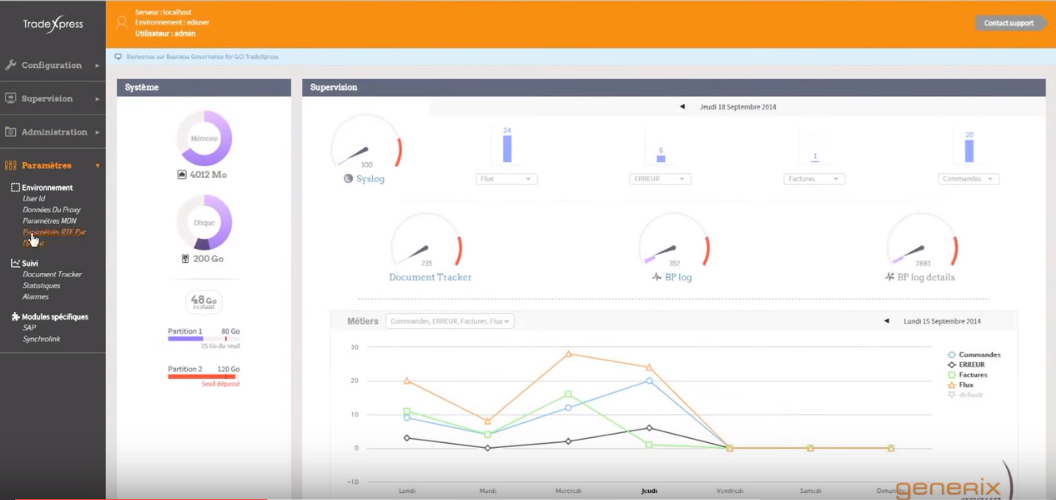
\includegraphics[width=17cm]{../img/part2/trade_xpress.png}
				\caption{\label{trade_xpress} Tableau de bord de l'outil Trade Xpress.}
			\end{figure}
			
			\paragraph{M12 :}
			M12 est une console permettant de monitorer des flux existant, principalement
			les flux basés sur des web services. La console permet de générer des
			alertes (par exemple des alertes mail) en cas de problème, et de rejouer les
			flux.
			\begin{figure}[h]
				\centering
				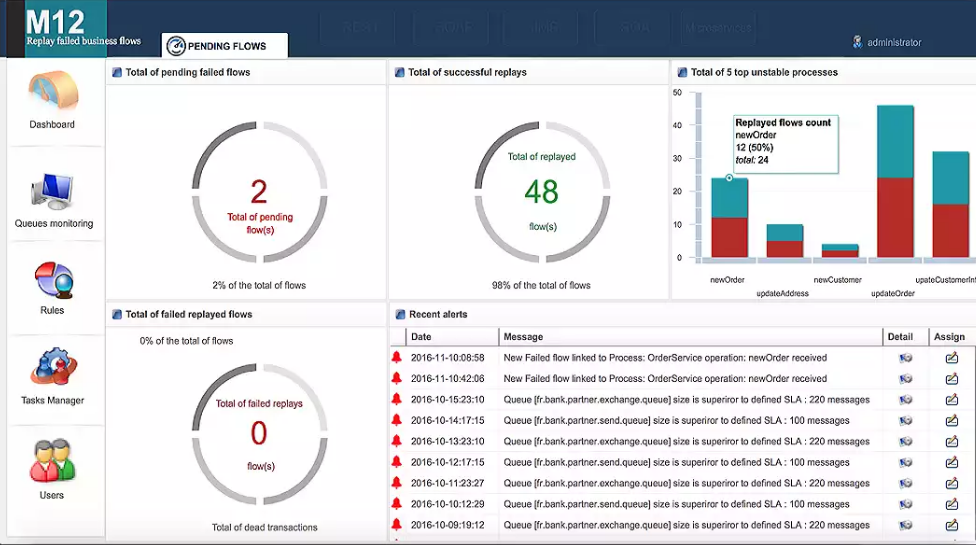
\includegraphics[width=17cm]{../img/part2/m12.png}
				\caption{\label{m12} Tableau de bord de l'outil M12.}
			\end{figure}
			
		\subsubsection{Choix des modes de visualisation par le biais de maquettes}
			\paragraph{}
			Texte de la sous sous partie
		\subsubsection{Création de scénarios d'utilisation}
			\paragraph{}
			Texte de la sous sous partie
